\documentclass{article}

%% PAQUETES

% Paquetes generales
\usepackage[margin=2cm, paperwidth=210mm, paperheight=297mm]{geometry}
\usepackage[spanish]{babel}
\usepackage[utf8]{inputenc}
\usepackage{gensymb}

% Paquetes para estilos
\usepackage{textcomp}
\usepackage{setspace}
\usepackage{colortbl}
\usepackage{color}
\usepackage{color}
\usepackage{upquote}
\usepackage{xcolor}
\usepackage{listings}
\usepackage{caption}
\usepackage[T1]{fontenc}
\usepackage[scaled]{beramono}

% Paquetes extras
\usepackage{amssymb}
\usepackage{float}
\usepackage{graphicx}
\usepackage{url}
\usepackage[toc,page]{appendix}
\usepackage{mips}


%% Fin PAQUETES


% Definición de preferencias para la impresión de código fuente.
%% Colores
\definecolor{gray99}{gray}{.99}
\definecolor{gray95}{gray}{.95}
\definecolor{gray75}{gray}{.75}
\definecolor{gray50}{gray}{.50}
\definecolor{keywords_blue}{rgb}{0.13,0.13,1}
\definecolor{comments_green}{rgb}{0,0.5,0}
\definecolor{strings_red}{rgb}{0.9,0,0}

%% Caja de código
\DeclareCaptionFont{white}{\color{white}}
\DeclareCaptionFont{style_labelfont}{\color{black}\textbf}
\DeclareCaptionFont{style_textfont}{\it\color{black}}
\DeclareCaptionFormat{listing}{\colorbox{gray95}{\parbox{16.78cm}{#1#2#3}}}
\captionsetup[lstlisting]{format=listing,labelfont=style_labelfont,textfont=style_textfont}

\lstset{
	aboveskip = {1.5\baselineskip},
	backgroundcolor = \color{gray99},
	basicstyle = \ttfamily\footnotesize,
	breakatwhitespace = true,   
	breaklines = true,
	captionpos = t,
	columns = fixed,
	commentstyle = \color{comments_green},
	escapeinside = {\%*}{*)}, 
	extendedchars = true,
	frame = lines,
	keywordstyle = \color{keywords_blue}\bfseries,
	language = C,                       
	numbers = left,
	numbersep = 5pt,
	numberstyle = \tiny\ttfamily\color{gray50},
	prebreak = \raisebox{0ex}[0ex][0ex]{\ensuremath{\hookleftarrow}},
	rulecolor = \color{gray75},
	showspaces = false,
	showstringspaces = false, 
	showtabs = false,
	stepnumber = 1,
	stringstyle = \color{strings_red},                                    
	tabsize = 2,
	title = \null, % Default value: title=\lstname
	upquote = true,                  
}

%% FIGURAS
\captionsetup[figure]{labelfont=bf,textfont=it}
%% TABLAS
\captionsetup[table]{labelfont=bf,textfont=it}

% COMANDOS

%% Titulo de las cajas de código
\renewcommand{\lstlistingname}{Código}
%% Titulo de las figuras
\renewcommand{\figurename}{Figura}
%% Titulo de las tablas
\renewcommand{\tablename}{Tabla}
%% Referencia a los códigos
\newcommand{\refcode}[1]{\textit{Código \ref{#1}}}
%% Referencia a las imagenes
\newcommand{\refimage}[1]{\textit{Imagen \ref{#1}}}

%% APENDICES
\addto\captionsspanish{
	\renewcommand\seename{Apéndices}
	\renewcommand\appendixname{Apéndices}
	\renewcommand\appendixpagename{Apéndices}
}


\begin{document}
\pagenumbering{roman}
\setcounter{page}{5}

% TÍTULO, AUTORES Y FECHA
\begin{titlepage}
	\vspace*{\fill}
	\begin{center}
		\huge{Trabajo Pŕactico N°1} \\
		\medskip
		\Huge \textit{``Conjunto de instrucciones MIPS''} \\
		
		\bigskip\bigskip\bigskip\bigskip\bigskip

		\Large Belén Beltran, Padrón Nro. 91.718 \\
		\large \textit{belubeltran@gmail.com} \\ \medskip
		\Large Pablo Ariel Rodriguez, Padrón Nro. 93.970 \\
		\large \textit{prodriguez@fi.uba.ar} \\ \medskip
		\Large Federico Martín Rossi, Padrón Nro. 92.086 \\
		\large \textit{federicomrossi@gmail.com} \\

		\bigskip\bigskip\bigskip\bigskip\bigskip\bigskip\bigskip

		\large 2do. Cuatrimestre 2013 \\ \smallskip
		\large 66.20 Organización de Computadoras \\ \smallskip
		\large Facultad de Ingeniería, Universidad de Buenos Aires \\ \smallskip

		\date{}
	\end{center}
	\vspace*{\fill}
\end{titlepage}

\newpage
\newpage \textit{}
\newpage



% ÍNDICE
\tableofcontents
\newpage \textit{}
\newpage
\pagenumbering{arabic}




% Introducción
\section{Introducción}
	
	En el presente trabajo se tiene como objetivo la comparación entre dos algoritmos de ordenamiento: el \textit{Bubblesort} y el \textit{Shellsort}.
	Para realizar dicha comparación entre ambos se realizó la implementación en lenguaje C de cada uno de estos. A su vez, para comparar el rendimiento entre código de alto nivel y de código nativo, se desarrollo la implementación del Heapsort en assembly MIPS, con el fin de poder comparar los tiempos de ejecución de ambos programas y realizar así un estudio de las mejoras que se producen.
	\par
	La totalidad del trabajo se ha realizado en una plataforma \textit{NetBSD/MIPS-32} mediante el \textit{GXEmul} \cite{GXEMUL}.
	\par
	Todos los archivos y códigos fuente aquí mencionados, así como también el presente informe, pueden ser descargados como un archivo comprimido ZIP del repositorio del grupo\footnote{URI del Repositorio: \url{https://github.com/federicomrossi/6620-trabajos-practicos-2C2013/tree/master/tp1}}.
\bigskip




% Compilación
\section{Compilación}
	
	
	La herramienta para compilar tanto el código asembly como C será el \textit{GCC} \cite{GCC}. Para tratar de equiparar al máximo el \textit{S} generado por ambas implementaciones, se utilizará el flag de gcc ``-O0'' para que no realice optimizaciones sobre el código en lenguaje C.
	\par
	Para automatizar las tareas de compilación se hace uso de la herramienta \textit{GNU Make}. Los Makefiles utilizados para la compilación se incluyen junto al resto de los archivos fuentes del presente trabajo \footnote{Los archivos se encuentran separados según la implemetación a la que pertenecen, por lo que habrán dos Makefiles distintos, uno para la implementación en lenguaje C y otro para la implementación en assembly}.
\bigskip




% Utilización
\section{Utilización}
	
	En los siguientes apartados se especifica la forma en la que deben ser ejecutados los programas implementados tanto en C como en assembly MIPS.



% Utilización - Implementación en C
\subsection{Implementación en C}

	El resultado de compilación utilizando el comando \textit{make} será un archivo ejecutable de nombre \textit{tp1}, que podrá ser invocado con los siguientes parámetros:
	\medskip

	\begin{itemize}

		\itemsep=2pt \topsep=0pt \partopsep=0pt \parskip=0pt \parsep=0pt
			\item \textit{-h}:  Imprime ayuda para la utilización del programa;
			\item \textit{-V}:  Imprimer la versión actual del programa;
			\item \textit{-b [ARGS]}:  El programa recibe nombres de archivos de texto o strings ingresados por \textit{stdin}, ordenandolos utilizando el algoritmo Bubblersort. Para utilizar \textit{stdin} deberá omitirse [ARGS] y luego introducir las palabras;
			\item \textit{-s [ARGS]}:  El programa recibe nombres de archivos de texto o strings ingresados por \textit{stdin}, ordenandolos utilizando el algoritmo Heapsort. Para utilizar \textit{stdin} deberá omitirse [ARGS] y luego introducir las palabras.

	\end{itemize}	
	\medskip



\subsection{Implementación en Assembly}

	El resultado de compilación utilizando el comando \textit{make} será un archivo ejecutable de nombre \textit{tp1}, el cual aceptará un archivo de texto como argumento y lo ordenará con el algoritmo Shellsort.
\medskip




% Implementación
\section{Implementación}
	
	En lo que sigue de la sección, se presentarán los códigos fuente de la implementación del algoritmo. Aquellos lectores interesados en la implementación completa del programa, pueden dirigirse al apéndic ubicado al final del presente informe.
\bigskip



% Implementación en C
\subsection{Implementación en C}

	La implementación del programa fue divida en los siguientes módulos:
	\medskip

\begin{itemize}

\itemsep=2pt \topsep=0pt \partopsep=0pt \parskip=0pt \parsep=0pt
	\item \textbf{tp1}: Programa principal responsable de interpretar los comandos pasados por la terminal de modo que realice las tareas solicitadas por el usuario. Su principal función es encadenar el funcionamiento de los otros módulos y mostrar por pantalla el resultado obtenido;
	\item \textbf{bubblesort}: Módulo encargado de implementar el algoritmo de ordenamiento Bubblesort. Recibe como parámetros un arreglo de palabras desordenado y el tamaño del mismo. Como resultado devuelve dicho arreglo ordenado.
	\item \textbf{heapsort}: Módulo encargado de implementar el algoritmo de ordenamiento Heapsort. Recibe como parámetros un arreglo de palabras desordenado y el tamaño del mismo. Como resultado devuelve dicho arreglo ordenado.

\end{itemize}	
\medskip


% Algoritmo Bubblesort 
\subsubsection{Algoritmo \textit{Bubblesort}}

	En el \refcode{codeBSh} se muestra el header de la librería, donde se declara la función \textit{bubblesort}, mientras que en el \refcode{codeBSc} se muestra la definición de la librería.

% Código
\lstset{ language = C } % Cambiamos el lenguaje para que parsee en C
\lstinputlisting[label=codeBSh,caption=``bubblesort.h'']{../codigo/c/bubblesort.h} 
\bigskip


% Código
\lstset{ language = C } % Cambiamos el lenguaje para que parsee en C
\lstinputlisting[label=codeBSc,caption=``bubblesort.c'']{../codigo/c/bubblesort.c} 
\bigskip\bigskip




% Algoritmo Shellsort
\subsubsection{Algoritmo \textit{Heapsort}}

	En el \refcode{codeHSh} se muestra el header de la librería, donde se declara la función \textit{heapsort}, mientras que en el \refcode{codeHSc} se muestra la definición de la librería.

% Código
\lstset{ language = C } % Cambiamos el lenguaje para que parsee en C
\lstinputlisting[label=codeHSh,caption=``heapsort.h'']{../codigo/c/heapsort.h} 
\bigskip


% Código
\lstset{ language = C } % Cambiamos el lenguaje para que parsee en C
\lstinputlisting[label=codeHSc,caption=``heapsort.c'']{../codigo/c/heapsort.c} 
\bigskip\bigskip



% Implementación en Assembly
\subsection{Implementación en Assembly}

	La implementación del programa fue divida en los siguientes módulos:
	\medskip

\begin{itemize}

\itemsep=2pt \topsep=0pt \partopsep=0pt \parskip=0pt \parsep=0pt
	\item \textbf{tp1}: Solamente recibe un texto como argumento por linea de comandos y lo imprime ordenandolo mediante heapsort. Esta implementado en  lenguaje C;
	\item \textbf{strcmpi}: Función implementada en assembly MIPS que se encarga de realizar la comparación de strings sin ser sensible a mayúsculas;
	\item \textbf{heap}: Función implementada en assembly MIPS que se encarga de [...];
	\item \textbf{heapsort}: Implementación en assembly MIPS del algoritmo de ordenamiento Heapsort.

\end{itemize}	
\medskip




% Algoritmo Heapsort
\subsubsection{Algoritmo \textit{Heapsort}}

	En el \refcode{codeHSaMED} se muestra la implementación en assembly del algoritmo Heapsort.

% Código
\lstset{ language = [mips]Assembler} % Cambiamos el lenguaje para que parsee en MIPS
\lstinputlisting[label=codeHSaMED,caption=``heapsort.S'']{../codigo/assembly/heapsort.S} 
\bigskip\bigskip\medskip



% Debugging
\section{Debugging}
	
	Para analizar el correcto funcionamiento del programa se crearon casos de prueba pertinentes, considerando combinaciones diferentes en el ingreso de parámetros al programa principal, como también tomando en cuenta las diferentes salidas obtenidas a partir del algorirmo \textit{pgm}. Los resultados fueron comparados con los casos esperados y así se determinó el correcto funcionamiento del programa en su totalidad.
\bigskip\bigskip




% Pruebas
\section{Pruebas}

\subsection{Pruebas al ingreso y egreso de datos del programa}
\medskip

	A modo de prueba del programa, se ingresaron ciertos parámetros a éste y se analizó la salida obtenida. A continuación se presentan algunas pruebas realizadas y los resultados obtenidos.
	\par
	El primer caso consiste en crear un tablero de resolución 11x16 y que el resultado sea enviado a la salida estandar. Se debe ingresar por consola lo siguiente:
	\bigskip

{\ttfamily\footnotesize
\indent \$ ./tp0 -r 11x16 -o -\\}
\smallskip

	La salida del programa es la siguiente:
	\bigskip

{\ttfamily\footnotesize
	\indent P2 \\
	\indent \# - \\
	\indent 11 16 \\
	\indent 1 \\
	\indent 1 1 0 0 1 1 0 1 0 1 0 \\
	\indent 1 1 0 0 1 1 0 1 0 1 0 \\
	\indent 0 0 1 1 0 0 1 0 1 0 1 \\ 
	\indent 0 0 1 1 0 0 1 0 1 0 1 \\ 
	\indent 1 1 0 0 1 1 0 1 0 1 0 \\ 
	\indent 1 1 0 0 1 1 0 1 0 1 0 \\ 
	\indent 0 0 1 1 0 0 1 0 1 0 1 \\ 
	\indent 0 0 1 1 0 0 1 0 1 0 1 \\ 
	\indent 1 1 0 0 1 1 0 1 0 1 0 \\ 
	\indent 1 1 0 0 1 1 0 1 0 1 0 \\ 
	\indent 0 0 1 1 0 0 1 0 1 0 1 \\ 
	\indent 0 0 1 1 0 0 1 0 1 0 1 \\ 
	\indent 1 1 0 0 1 1 0 1 0 1 0 \\ 
	\indent 1 1 0 0 1 1 0 1 0 1 0 \\ 
	\indent 0 0 1 1 0 0 1 0 1 0 1 \\ 
	\indent 0 0 1 1 0 0 1 0 1 0 1 \\ 
}
\bigskip


	La segunda prueba consiste en crear un tablero de resolución 16x11 y también enviar la salida a consola. Se debe ingresar por la línea de comandos:
	\bigskip

{\ttfamily\footnotesize
\indent \$ ./tp0 -r 16x11 -o -\\}
\smallskip

	La salida del programa es la siguiente:
	\bigskip

{\ttfamily\footnotesize
	\indent P2 \\
	\indent \# - \\
	\indent 16 11 \\
	\indent 1 \\
	\indent 1 1 0 0 1 1 0 0 1 1 0 0 1 1 0 0 \\
	\indent 1 1 0 0 1 1 0 0 1 1 0 0 1 1 0 0 \\
	\indent 0 0 1 1 0 0 1 1 0 0 1 1 0 0 1 1 \\
	\indent 0 0 1 1 0 0 1 1 0 0 1 1 0 0 1 1 \\
	\indent 1 1 0 0 1 1 0 0 1 1 0 0 1 1 0 0 \\
	\indent 1 1 0 0 1 1 0 0 1 1 0 0 1 1 0 0 \\
	\indent 0 0 1 1 0 0 1 1 0 0 1 1 0 0 1 1 \\
	\indent 1 1 0 0 1 1 0 0 1 1 0 0 1 1 0 0 \\
	\indent 0 0 1 1 0 0 1 1 0 0 1 1 0 0 1 1 \\
	\indent 1 1 0 0 1 1 0 0 1 1 0 0 1 1 0 0 \\
	\indent 0 0 1 1 0 0 1 1 0 0 1 1 0 0 1 1 \\
}
\bigskip


	La tercer prueba consiste en generar el tablero de tamaño default 8x8 (se genera en caso de no ingresar la opción -r), ingresando por consola:
	\bigskip

{\ttfamily\footnotesize
\indent \$ ./tp0 -o -\\}
\smallskip

	El resultado del programa se ve por salida standard y es el siguiente:
	\bigskip

{\ttfamily\footnotesize
	\indent P2 \\
	\indent \# - \\
	\indent 8 8 \\
	\indent 1 \\
	\indent 1 0 1 0 1 0 1 0 \\
	\indent 0 1 0 1 0 1 0 1 \\
	\indent 1 0 1 0 1 0 1 0 \\
	\indent 0 1 0 1 0 1 0 1 \\
	\indent 1 0 1 0 1 0 1 0 \\
	\indent 0 1 0 1 0 1 0 1 \\
	\indent 1 0 1 0 1 0 1 0 \\
	\indent 0 1 0 1 0 1 0 1 \\
}
\bigskip


	Una prueba más interesante, es aquella en la cual la resolución permite ver una imagen bastante amplia. En este caso se considera una resolución de 200x200 y se decide guardar la salida en un archivo. Se debe ingresar por consola:
	\bigskip

{\ttfamily\footnotesize
\indent \$ ./tp0 -r 200x200 -o 200x200.pgm\\}
\smallskip

	La salida en formato de imagen \textit{PGM} se muestra en la \textit{Figura 1}.


\newpage
%\begin{figure}[H]
%	\centering
%	
\includegraphics[width=0.36\textwidth]{images/200x200.jpg}
%	\medskip
%	\caption{Imágen del tablero de ajedrez con resolución de 200x200 píxeles.}
%\end{figure}
%\bigskip\bigskip


\subsection{Tiempos de ejecución}

	\par
	Se quiere medir el tiempo que tarda el programa en la máquina virtual MIPS32 en crear un tablero de ajedrez con ciertas características. Para ello se realizó un módulo aparte que, con la ayuda del comando \textit{GNU ``time''} \cite{TIME}, mide los tiempos de la realización de un tablero de resolución 1x1 hasta uno de 1000x1000. 
	\par
	Los datos obtenidos se pueden observar en el \textit{Cuadro 1}. 
	\bigskip\bigskip


% Tabla 1
\begin{table}[!hbt]
	\begin{center}
	\begin{tabular}{|>{\centering\arraybackslash}m{3cm}|>{\centering \arraybackslash}m{3cm}|}
		\hline
		\rowcolor[gray]{0.9}\textbf{Resolución} & \textbf{Tiempo de ejecución [s]}\\
		\hline
		\centering 1x1 & 0,051 \\
		\hline
		\centering 100x100 & 0,316 \\
		\hline
		\centering 200x200 & 1,148 \\
		\hline
		\centering 300x300 & 2,5 \\
		\hline
		\centering 400x400 & 4,434 \\
		\hline
		\centering 500x500 & 6,844 \\
		\hline
		\centering 600x600 & 9,848 \\
		\hline
		\centering 700x700 & 13,5 \\
		\hline
		\centering 800x800 & 17,449 \\
		\hline
		\centering 900x900 & 22,152 \\
		\hline
		\centering 1000x1000 & 27,613 \\
		\hline
	\end{tabular}
	\smallskip
	\caption{Tiempos en segundos obtenidos en la ejecución\\ del programa para distintas resoluciones.}
	\end{center}
\end{table}
\bigskip\bigskip


	En la \textit{Figura 2} se presenta un diagrama resumido de los tiempos de ejecución obtenidos. Como es de esperar, se obtiene una curva cuadrática.


\newpage	
% Figura 2
%\begin{figure}[h]
%	\centering
%	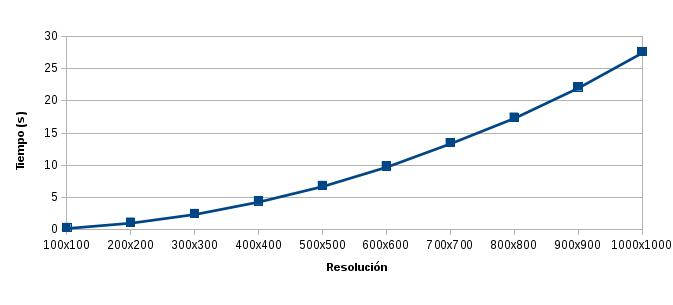
\includegraphics[width=1.0\textwidth]{images/grafico-tiempos.jpg}
%	\caption{Gráfico de tiempo de ejecución (en segundos) respecto\\ de la resolución de imagen generada.}
%\end{figure}
%\bigskip\bigskip\bigskip




% Citas bibliográficas.
\begin{thebibliography}{99}

	\bibitem{GXEMUL} The NetBSD project, \url{http://www.netbsd.org/}

	\bibitem{GCC} GCC, the GNU Compiler Collection, \url{http://gcc.gnu.org/}

	\bibitem{BS} PGM format speciffication, \url{http://netpbm.sourceforge.net/doc/pgm.html}

	\bibitem{TIME} time man page, \url{http://unixhelp.ed.ac.uk/CGI/man-cgi?time}

	\bibitem{HEN00} J. L. Hennessy and D. A. Patterson, ``Computer Architecture. A Quantitative
	Approach,'' 4th Edition, Morgan Kaufmann Publishers, 2000.

	\end{thebibliography}

\newpage


% Apendices
\begin{appendices}

\bigskip\bigskip

% Implementación completa en lenguaje C
\section{Implementación completa en lenguaje C}


\subsection{\textit{tp0.c}. Implementación del main del programa}
% Código
%\lstset{ language = C } % Cambiamos el lenguaje para que parsee en C
%\lstinputlisting[label=codeTP0cfull,caption=``tp0.c'']{../codigo/tp0.c} 
%\bigskip\bigskip

\subsection{\textit{pgm.h}. Declaración de la librería Pgm}
% Código
%\lstset{ language = C } % Cambiamos el lenguaje para que parsee en C
%\lstinputlisting[label=codeBShfull,caption=``pgm.h'']{../codigo/pgm.h} 
%\bigskip\bigskip

\subsection{\textit{pgm.c}. Definición de la librería Pgm}
% Código
%\lstset{ language = C } % Cambiamos el lenguaje para que parsee en C
%\lstinputlisting[label=codeBScfull,caption=``pgm.c'']{../codigo/pgm.c} 
%\bigskip\bigskip



% Implementación completa en assembly MIPS
\section{Generación del código completo en assembly MIPS}


\subsection{\textit{tp0.s}. Generación del main del programa}
% Código
%\lstset{ language = [mips]Assembler } % Cambiamos el lenguaje para que parsee en C
%\lstinputlisting[label=codeTP0afull,caption=``tp0.s'']{../codigo/tp0.s} 
%\bigskip\bigskip

\subsection{\textit{pgm.s}. Generación del algoritmo Pgm}
% Código
%\lstset{ language = [mips]Assembler} % Cambiamos el lenguaje para que parsee en MIPS
%\lstinputlisting[label=codeSSafull,caption=``pgm.s'']{../codigo/pgm.s} 
%\bigskip\bigskip


\end{appendices}

\end{document}
